% INTRODUCCIÓN

\cleardoublepage

\chapter{Introducción}
\label{introduccion}

El objetivo es poder realizar el seguimiento a tiempo real de una persona a través de la cámara del dispositivo utilizando para ello visión por computador y técnicas de aprendizaje por refuerzo para controlar las acciones a tomar en cada momento. Lo que se conoce como active tracking. 
\medskip

Los actuales algoritmos se centran fundamentalmente en el reconocimiento del objeto y en la posición de éste con respecto a las coordenadas X e Y en relación al centro de la imagen a través de la cámara incorporada para guiar las acciones del dispositivo. Es lo que se conoce como \textit{passive tracking}. Este tipo de algoritmos han ganado más atención debido a la simplicidad del problema y los avances en reconocimiento de objetos.
\medskip

Otros intentos de realizar \textit{object tracking} con aprendizaje supervisado se realizan utilizando modelos en simuladores tanto del dron como de las personas. Sin embargo, la idea del presente trabajo es la aplicación de diferentes técnicas de inteligencia artificial para lograr un agente que sea capaz de realizar el seguimiento utilizando simplemente imágenes que provengan del propio dispositivo en el cual se desplegará el agente.
\medskip

\begin{figure}[ht!]
\centering
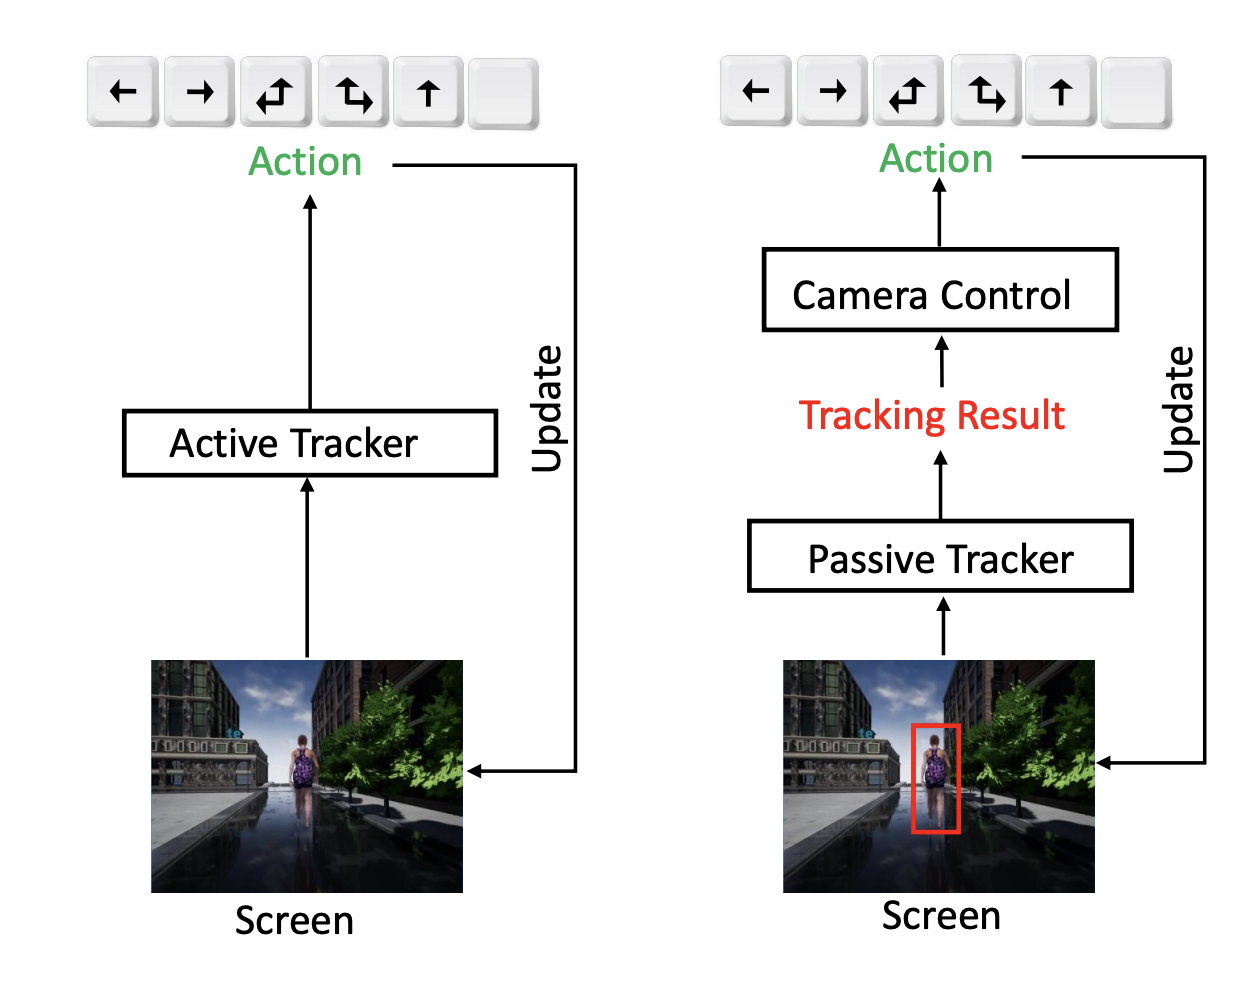
\includegraphics[scale=0.4]{figuras/active_tracking_vs_passive_tracking.png}
\caption[A la izquierda, el pipeline utilizado durante active tracking. A la derecha, el pipeline utilizado en passive tracking.]{A la izquierda, el pipeline utilizado durante active tracking. A la derecha, el pipeline utilizado en passive tracking. Imagen tomada de \citet{luo2019end}.}
\label{fig-active-tracking}
\end{figure}
\medskip

Para ello, no solo utilizaremos técnicas de aprendizaje por refuerzo, sino también técnicas de aprendizaje supervisado para la obtención de nuestro conjunto inicial.
\medskip

El desarrollo del proyecto se llevará a cabo utilizando lenguaje Python y la librería \href{https://pytorch.org/}{PyTorch} para el desarrollo de los modelos. El código completo estará disponible para su visualización en un repositorio de \href{https://github.com/lucaswerner90/msc-degree-ai}{GitHub}, a excepción de los pesos de los diferentes agentes que se vayan guardando durante el entrenamiento debido al tamaño individual de cada uno de estos archivos.


\section{Acotación del problema}
\label{acotacion-del-problema}

Debido a que nos movemos en un entorno real, en el cual las posibilidades son muy amplias, no solo debido a la aleatoriedad del mismo sino también al número de acciones que podemos tomar, debemos definir ciertas restricciones.
\medskip

En primer lugar, nos centraremos en obtener una solución que sea viable en entornos en los cuales las condiciones externas no sean un impedimento para el buen funcionamiento de nuestro algoritmo. Esto quiere decir que durante el desarrollo y testeo de los algoritmos obviamos factores tales como el viento, las condiciones de humedad o el grado de iluminación en un momento dado, que pudiesen afectar al rendimiento del dispositivo.
\medskip

Por otro lado, debido a que el espacio de acciones disponibles es muy alto, en una primera fase dispondremos de tan solo 3: 

\begin{itemize}
  \item Girar a la derecha.
  \item Girar a la izquierda.
  \item Mantenerse en el mismo lugar.
\end{itemize}
\medskip

Tanto el giro a la derecha como el giro a la izquierda se realizará en el dispositivo de manera controlada, esto quiere decir que nos moveremos siempre utilizando el mismo ángulo de giro. Si quisiéramos añadir además un ángulo de giro variable junto con la acción a tomar podríamos hacerlo como parte de la salida de nuestro algoritmo, aunque involucraría un entrenamiento más prolongado en el tiempo y se escaparía a las restricciones de tiempo de este proyecto.
\medskip

De tal forma que nuestra solución será valorada positiva o negativamente con respecto al eje X exclusivamente. Esto quiere decir que consideraremos que el algoritmo funciona de forma correcta si es capaz de moverse de tal manera que la persona se encuentre siempre centrada en el eje horizontal y no en el eje vertical.
\medskip

En cuanto a la detección de la persona, tenemos en cuenta que nuestro dispositivo solo realizará el seguimiento de una sola persona, debido a la complejidad que esto supondría en cuanto al funcionamiento de nuestro algoritmo. Obviamos un escenario real y plausible que es el de encontrarnos en una misma imagen con múltiples personas, en cuyo caso deberíamos también de desarrollar un mecanismo de selección de la persona a la cual quisiéramos seguir.
\medskip

Por lo tanto, quedándonos con una parte simplificada del problema, podemos centrarnos en conseguir un algoritmo que pueda considerarse como el mínimo viable para conseguir nuestro objetivo.
\medskip

\section{Dispositivo utilizado}
\label{dispositivo-utilizado}

Para el desarrollo del proyecto se utilizará el dispositivo DJI Tello, ya que nos proporciona una interfaz de programación compatible con nuestras necesidades: control del dispositivo y transmisión de datos a través de una API en lenguaje Python.
\medskip


\begin{figure}[ht!]
  \centering
  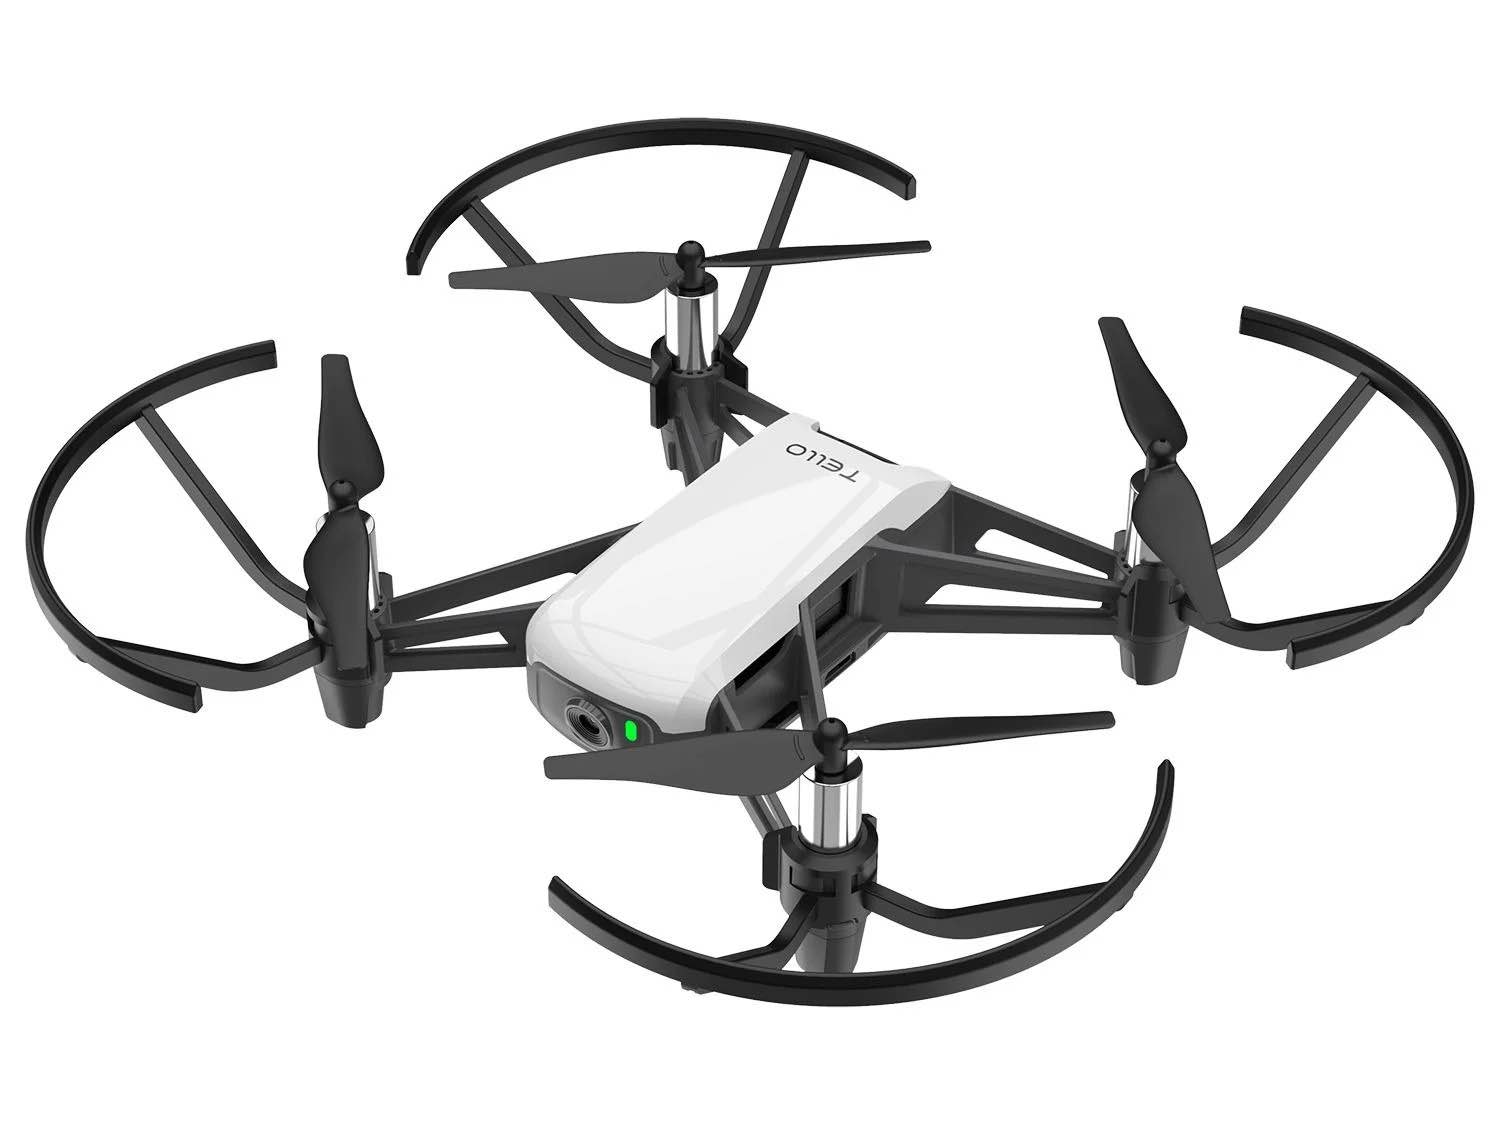
\includegraphics[scale=0.2]{figuras/dispositivo_utilizado.png}
  % \caption[Así aparece el rótulo en el índice]{Así aparece el rótulo en el texto.}
  \caption[DJI Tello. Dispositivo utilizado durante el proyecto]{Imagen del dispositivo utilizado durante el proyecto.}
  \label{fig-dron}
\end{figure}


El dispositivo cuenta con una cámara integrada con una resolución máxima de 1280x720 píxeles, la cual creemos que es suficiente para el desarrollo del trabajo.
\medskip

Un punto negativo del uso de drones como dispositivo de captura es el poco rendimiento de las baterías durante el vuelo. Concretamente, el dron utilizado permanece en vuelo unos 13 minutos como máximo.
\medskip

Además, durante el desarrollo inicial del proyecto se pudo observar una latencia reseñable al intentar comunicar el dispositivo con el ordenador a la hora de transmitir las imágenes y de poder enviar señales de control debido a la débil conexión WiFi entre ambos puntos de comunicación. El intentar solucionar este problema no solo consumió tiempo de ejecución del proyecto sino que también nos impide poder llevar a cabo pruebas de control más realistas y nos acotará el margen de ejecución de nuestras pruebas finales.
\medskip

\section{Marco teórico}

En esta sección haremos una breve introducción a los diferentes componentes teóricos que nos iremos encontrando a lo largo del trabajo. Empezaremos repasando los principales conceptos relacionados con el aprendizaje por refuerzo y en qué se diferencia de otros tipos de entrenamiento. 
\medskip

Después haremos una introducción a cada uno de los algoritmos que vamos a utilizar y comentaremos brevemente las diferencias y el por qué los elegimos.
Por último comentaremos los \textit{Transformers}\citep{transformers} y en especial los \textit{Vision Transformers}\citep{visiontransformers}, ya que serán utilizados durante uno de los experimentos que explicaremos en la sección \ref{resultados-y-discusion} .
\medskip

\subsection{Aprendizaje por refuerzo}
\label{aprendizaje-por-refuerzo}

\subsection{Algoritmo Policy Gradient}
\label{algoritmo-policy-gradient}

\subsection{Algoritmo Actor Critic}
\label{algoritmo-actor-critic}

\subsection{Vision Transformers}
\label{vision-transformers}
